\title{LEZIONE 11 12/05/2020}\newline
\textbf{link} \href{https://web.microsoftstream.com/video/5bd1efee-fafa-4133-8e33-37fcd8b66da5}{clicca qui}
\subsection{Attrito dinamico o radente}
Nel momento in cui viene applicata una forza $F$ su un corpo e che la forza di attrito $T$ non è più in grado di bilanciarla si instaura un moto relativo fra i due corpi a contatto.\newline
\newline
Per verificare se si instaura o meno un moto relativo di usa la \textbf{verifica di aderenza}, cioè:
\[
    T \leq T_{lim} = f_s N
\]
Se questa disequazione si verifica siamo in presenza di \textbf{attrito statico}, se non si verifica siamo in condizione di \textbf{attrito dinamico}.\newline
\newline
In condizioni di attrito dinamico, il modello di Coulomb ci permette di stabilire la forza $T$ (o meglio $T_1$ e $T_2$ per effetto di azione-reazione) che viene scambiata fra i due corpi a contatto:\newline
[immagine dagli appunti del prof]
\begin{center}
    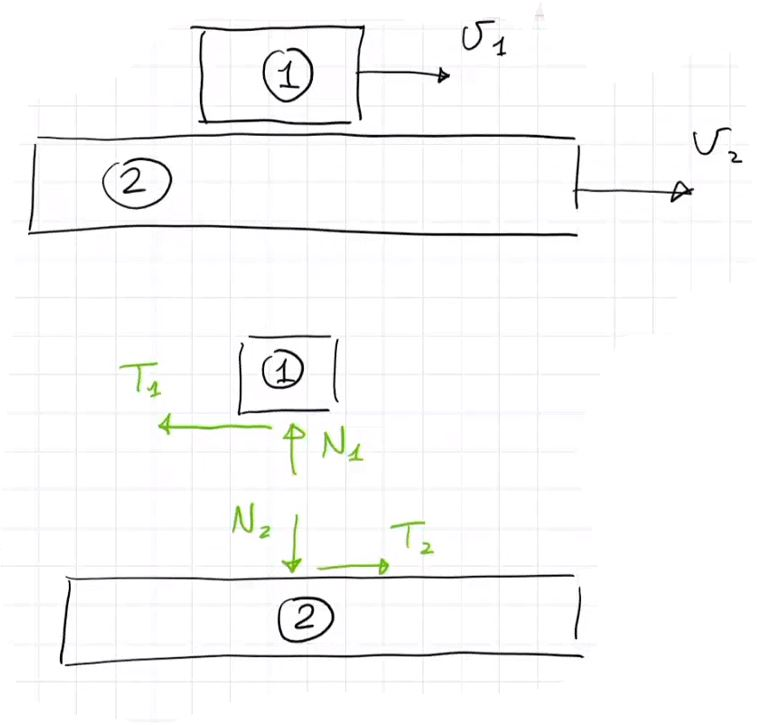
\includegraphics[height=3cm]{../lezione11/img1.JPG}
\end{center}
\[
    \begin{cases}
        \vec{T}_1 = - \vec{T}_2\\
        \vec{N}_1 = - \vec{N}_2
    \end{cases} \rightarrow \begin{cases}
        |\vec{T}_1| = |\vec{T}_2| = T\\
        |\vec{N}_1| = |\vec{N}_2| = N
    \end{cases}
\]
Possiamo ora definire la forza di attrito per il primo corpo come:
\[
    \vec{T}_1 = - f_d N  \frac{\vec{v}_{12}}{|\vec{v}_{12}|} = - f_d N  \frac{\vec{v}_1 - \vec{v}_2}{|\vec{v}_1 - \vec{v}_2|} 
\]
con $f_d$ \textbf{coefficiente di attrito dinamico}, e modulo $ |\vec{T}_1| = f_d N$, mentre direzione $ - \frac{\vec{v}_{12}}{|\vec{v}_{12}|}$ opposta alla velocità di strisciamente del corpo $1$ rispetto al copro $2$, che può essere espresso anche come $\frac{\vec{v}_1 - \vec{v}_2}{|\vec{v}_1 - \vec{v}_2|}$.\newline
[immaigne dagli appunti del prof]
\begin{center}
    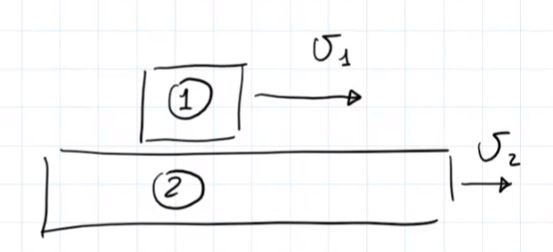
\includegraphics[height=3cm]{../lezione11/img2.JPG}
\end{center}
Notiamo inoltre che $\vec{v}_{12} = - \vec{v}_{21}$ e quindi la formula può essere riscritta come $\vec{T}_1 = f_d N  \frac{\vec{v}_{21}}{|\vec{v}_{21}|}$ .\newline
Porre molta attenzione a questo concetto di velocità relativa, la forza di attrito non dipende dalla velocità di uno solo dei due corpi, ma dalla velocità relativa di entrambi.
\ \newline
Operativamente il termine $N$ viene ricavato imponendo delle equazioni di equilibrio. Il termine $f_d$, che consideremo costante, dipende unicamente dai materiali a contatto, dalla finitura e dall'eventuale presenza di lubrificante. In realtà per velocità relative molto basse, il coefficiente di attrito dinamico non è costante e solitamente $f_d \leq f_s$.\newline
\newline
\subsubsection{Casi particolari}
Ipotiziamo che la velocità del corpo $2$ sia nulla: $\vec{v}_2 = 0$.\newline
[immaigne dagli appunti del prof]
\begin{center}
    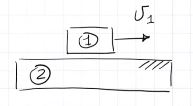
\includegraphics[height=3cm]{../lezione11/img3.JPG}
\end{center}
La forza di attrito sul corpo $1$ vale $|\vec{T}_1| = f_d N$ e la direzione sarà opposta alla velocità, cioè direzione $- \frac{\vec{v}_1}{|\vec{v}_1|}$. Sul secondo corpo quindi apparirà una forza uguale e contraria.\newline
[immagine dagli appunti del prof]
\begin{center}
    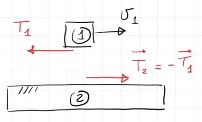
\includegraphics[height=3cm]{../lezione11/img4.JPG}
\end{center}
\ \newline
Ipotiziamo ora il caso contrario, cioè quello in cui $\vec{v}_1 = 0$:\newline
[immagine dagli appunti del prof]
\begin{center}
    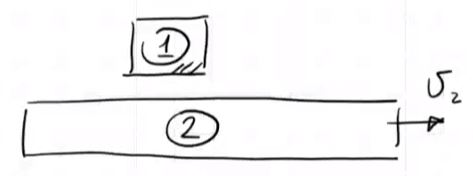
\includegraphics[height=3cm]{../lezione11/img5.JPG}
\end{center}
In questo caso, abbiamo sempre $|\vec{T}_1| = f_d N$, ma la direzione sarà contraria alla direzione di $\vec{v}_{12} = \vec{v}_1 - \vec{v}_2 = - \vec{v}_2$, per cui $\vec{T}_1 = - f_d N \frac{\vec{v}_2}{|\vec{v}_2|}$, quindi in questo caso $T_1$ avrà direzione concorde con $v_2$:\newline
[immagine dagli appunti del prof]
\begin{center}
    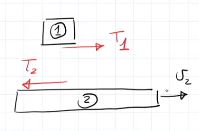
\includegraphics[height=3cm]{../lezione11/img6.JPG}
\end{center}